\documentclass{article}
\usepackage[english]{babel}
\usepackage{longtable}
\usepackage[top=1in, bottom=0.25in, left=1.25in, right=1.25in,includefoot,heightrounded]{geometry}
\usepackage{indentfirst}
\usepackage[utf8]{inputenc}
\usepackage{amsmath,amssymb}
\usepackage{graphicx,tikz}
\usepackage{hyperref}
\usepackage[colorinlistoftodos]{todonotes}
\usepackage[document]{ragged2e}
\usepackage{fancyhdr}
\usepackage{enumerate}
\usepackage{listings}
\usepackage{color}
\usepackage{flowchart}
\usepackage{hyperref}
\usepackage{graphicx}
\usetikzlibrary{arrows}

\usetikzlibrary{shapes.geometric, arrows}
\tikzstyle{startstop} = [rectangle, rounded corners, minimum width=3cm, minimum height=1cm,text centered, draw=black, fill=red!30]
\tikzstyle{decision} = [diamond, minimum width=4cm, minimum height=0.5cm, text centered, draw=black, fill=green!30]
\tikzstyle{process} = [rectangle, minimum width=3cm, minimum height=1cm, text centered, draw=black, fill=orange!30]
\tikzstyle{arrow} = [thick,->,>=stealth]
\tikzstyle{io} = [trapezium, trapezium left angle=70, trapezium right angle=110, minimum width=2cm, text width=4cm, minimum height=1cm, text centered, draw=black, fill=blue!30]

\pagestyle{fancy}
\fancyhf{}
\lhead{Myles Deslippe}
\rhead{Comp 3670 | Computer Networks}
\cfoot{\thepage}

\definecolor{MyDarkGreen}{rgb}{0.0,0.4,0.0}
\lstset{inputencoding=ansinew}
\lstset{breaklines=true} 

\begin{document}

    \section*{\centering{The Link Layer}}

    \subsection*{Introduction to the Link Layer}
    \begin{itemize}
        \item The \textbf{link layer} is responsible for \textbf{transferring datagrams} from one \textbf{node} to another \textbf{physically adjacent} node over a \textbf{link}.
        \item When working at the \textbf{link layer}, we refer to \textbf{hosts and routers} as \textbf{nodes}.
        \item When working at the \textbf{link layer}, we refer to \textbf{communication channels} that \textbf{connect adjacent nodes} as \textbf{links}.
        \begin{itemize}
            \item These links can be wired and wireless.
        \end{itemize}
        \item When working at the \textbf{link layer}, \textbf{frames} are the \textbf{unit of data} we are interested in \textbf{transferring}; they \textbf{encapsulate packets}.
        \item Different \textbf{types of links} have \textbf{different transfer protocols}. Different protocols provice different services (eg one may be reliable, the other may not be reliable).
    \end{itemize}

    \subsection*{Link Layer Services}
    \begin{itemize}
        \item The \textbf{framing service} is responsible for \textbf{encapsulating datagrams} into frames (adding headers, etc). If there is a shared medium, the channel access needs to be specified. MAC addresses are used in frame headers to identify devices.
        \item The \textbf{reliable deliver service} is responsible for ensuring \textbf{every frame is correctly delivered}.
        \item The \textbf{flow control service} is responsible for \textbf{pacing sending and receiving rates}.
        \item The \textbf{error detection service} is responsible for \textbf{detecting errors} caused by frame drops, noise, signal attenuation, etc.
        \item The \textbf{error correction service} is responsible for \textbf{identifying incorrect bits, and correcting them} without the need for retransmission.
        \item With a \textbf{half-duplex service} both nodes can transmit and receive, but not both operations at the same time.
        \item With a \textbf{full-duplex service} both nodes can transmit and receive at the same time.
    \end{itemize}

    \subsection*{Link Layer Implementation}
    \begin{itemize}
        \item The \textbf{link layer} is \textbf{implemented} in \textbf{each and every node}.
        \item \textbf{Implementations} are located in the node's \textbf{Network Interface Card (NIC)}. These cards implement the link and physical layer.
        \item The \textbf{implementations} are \textbf{connected} to the \textbf{system's bus} which allow for data transfer. And a combination of \textbf{hardware, software, and firmware control the NIC}.
    \end{itemize}

    \subsection*{Error Detection}
    \begin{itemize}
        \item An \textbf{Error Correction and Detection (EDC) bit} is used.
        \item If an \textbf{error is detected}, the device will either \textbf{correct the error}, or request a \textbf{retransmission}.
        \item \textbf{Error detection} is not 100\% reliable, but it is still useful. Larger EDC fields result in better detection and correction.
        \item \textbf{Parity checking} is also used.
        \item \textbf{Cyclic Redundancy Check (CRC)} is a good way of \textbf{detecting errors}.
    \end{itemize}

    \subsection*{Multiple Access Protocols}
    \begin{itemize}
        \item There are two types of links:
        \begin{enumerate}
            \item \textbf{Point-To-Point} | Two devices connected directly by a link (for example ethernet between two devices).
            \item \textbf{Broadcast} | Several devices connected by a shared medium that can communicate (for example a shared wire, a shared radio, a switch).
            \item When \textbf{two or more} nodes \textbf{simultaneously transmit}, \textbf{interference can occur}.
            \item \textbf{Collision occurs} if a \textbf{single node} receives \textbf{two or more signals at the same time}.
            \item There are \textbf{protocols} to \textbf{avoid interference and collision}; they involve a \textbf{distributed algorithm} that determins \textbf{how nodes share a channel}.
            \item \textbf{Communication} about \textbf{how to use a channel} must be \textbf{on the channel}, out-of-band coordination is not allowed in these protocols.
        \end{enumerate}
    \end{itemize}

    \subsection*{The Media Access Control (MAC) Protocol}
    \begin{itemize}
        \item In the \textbf{MAC protocol}, there are \textbf{three classifications of channel access control}:
        \begin{enumerate}
            \item \textbf{Channel Partitioning} | Channels are divided into smaller pieces (time slots, requency, code, etc), and pieces of the channel are allocated to nodes for exclusive use.
            \item \textbf{Random Access} | Channels are not divided, and allow collision, and provides a way to recover from collisions.
            \item \textbf{Taking Turns} | Nodes take turns using the channel, but nodes with more to send can take longer turns.
        \end{enumerate}
    \end{itemize}

    \subsection*{MAC Channel Partitioning Protocols}
    \begin{itemize}
        \item \textbf{Time Division Multiple Access (TDMA)} gives nodes access to the channel in \textbf{rounds}, each node gets a \textbf{fixed length slot} (length = packet transmission time) in each round.
        \begin{itemize}
            \item Unused slots go idle.
        \end{itemize}
        \item \textbf{Frequency Division Multiple Access (FDMA)} divides the channel into \textbf{frequency bands}, and each nodes gets a \textbf{fixed frequency band}.
        \begin{itemize}
            \item Unused frequency bands go idle.
        \end{itemize}
    \end{itemize}

    \subsection*{MAC Channel Random Access Protocols}
    \begin{itemize}
        \item When a \textbf{node has a packet to send}, it transmits to the \textbf{full channel} at a data rate $R$ \textbf{without any prior coordination}.
        \item If \textbf{two nodes transmit} at the \textbf{same time}, \textbf{collision occurs}.
        \item The \textbf{Random Access protocol} specifies how to \textbf{detect and recover} from \textbf{collisions}.
        \item Exampels of \textbf{Random Access protocols}: 
        \begin{enumerate}
            \item \textbf{ALOHA}:
            \begin{itemize}
                \item Assumptions: 
                \begin{enumerate}
                    \item All frames are the same size.
                    \item Time is divided into equal size transmission slots.
                    \item Nodes can only start transmitting at a slot beginning.
                    \item The nodes are all time-synchronized.
                    \item If two or more nodes transmit in a slot, all nodes detect the collision.
                \end{enumerate}
                \item When a node obtains a fresh frame, it will transmit it in the next slot, if collision occurs, retransmit, otherwise send the next frame.
                \item Suppose N nodes with many frames to send, each transmit in a slot with probability $P$, each time a node attempts to transmit, 37\% ($\frac{100}{e}$\%) of the time, nodes will be able to transmit without collision.
                \item Pros:
                \begin{enumerate}
                    \item Single active node can continuously transmit at full rate.
                    \item Highly decentralized.
                    \item Simple.
                \end{enumerate}
                \item Cons:
                \begin{enumerate}
                    \item Collision occurs, wasting time slots.
                    \item Some slots are idle.
                    \item Nodes may be able to detect collision in lass than time to transmit a packet.
                    \item Clock synchronization is difficult.
                \end{enumerate}
            \end{itemize}
            \item \textbf{Pure ALOHA}:
            \begin{itemize}
                \item \textbf{Pure ALOHA} is \textbf{ALOHA without the timeslots}. When a frame first arrives, nodes can attempt to transmit it immediately.
                \item The probability for collision increases with no synchronization.
                \item Suppose N nodes with many frames to send, each transmit with probability $P$, each time a node attempts to transmit, 18\% ($\frac{100}{2e}$\%) of the time, nodes will be able to transmit without collision.
            \end{itemize}
            \item \textbf{Simple Carrier Sense Multiple Access (Simple CSMA)}:
            \begin{itemize}
                \item CSMA requires nodes to listen before they transmit. If the channel is idle, they can transmit the entire frame. If the channel is busy, they can defer the transmission.
            \end{itemize}
            \item \textbf{CSMA/CD}:
            \begin{itemize}
                \item \textbf{CSMA/CD} is \textbf{Simple CSMA} with \textbf{Collision Detection}.
                \item Collision can be detected within a short period of time.
                \item Colliding transmissions are aborted, and rescheduled, reducing channel waste.
                \item Collision detection is easy in wired links, but difficult in wireless links.
                \item \textbf{CSMA/CD} is more efficient than \textbf{ALOHA}.
            \end{itemize}
        \end{enumerate}
    \end{itemize}

    \subsection*{MAC Taking Turns Protocols}
    \begin{itemize}
        \item \textbf{Taking turns} uses \textbf{polling}, a \textbf{master} invites \textbf{other nodes to transmit in turn}.
        \item Concerns with this type of protocol are: polling overhead, latency, and a single point of failiure (master).
        \item Another way to implement taking turns is with \textbf{token passing}. A \textbf{control token} is \textbf{passed sequentially} from \textbf{one node to the next}.
        \item Concerns with token passing are: token overhead, latency, single point of failiure (token).
    \end{itemize}

    \section*{\centering{Local Area Networks (LANs)}}

    \subsection*{MAC Addresses}
    \begin{itemize}
        \item A \textbf{MAC Address} is a \textbf{48-bit number} that \textbf{uniquely identifies} a \textbf{Network Interface Controller (NIC)}.
        \item \textbf{MAC Address allocation} is adiministered by \textbf{IEEE}. \textbf{Manufacturers} buy \textbf{MAC Address ranges} and assign those to devices they make (this is done to ensure uniqueness).
        \item \textbf{MAC Addresses} are used on \textbf{layer 2}.
    \end{itemize}

    \subsection*{The Address Resolution Protocol (ARP)}
    \begin{itemize}
        \item The \textbf{Address Resolution Protocol (ARP)} is a \textbf{communication protocol} that is used for \textbf{discovering} the \textbf{link-layer address of devices}.
        \item \textbf{ARP} is a \textbf{request-response protocol}, where messages are directly encapsulated by a link layer protocol. Such messages are \textbf{only communicated within the boundaries of a single network}, they are never routed across internetworking nodes.
        \item \textbf{Each IP node} on a \textbf{local area network} has an \textbf{ARP table}. These tables are used to maintain a \textbf{mapping} between each \textbf{MAC address} and it's corresponding \textbf{IP addresses}.
        \item \textbf{ARP table entries} consist of: \textbf{a MAC address, IP Addresses, and a TTL}.
        \item To find the \textbf{MAC Address of a node}, the following must be done:
        \begin{enumerate}
            \item The request node \textbf{broadcasts an ARP query} containing the \textbf{target node's IP addres}. The \textbf{target MAC Address field} in the request is set to \textbf{FF:FF:FF:FF:FF:FF} (which broadcasts it to all devices in the local network).
            \item \textbf{All nodes} receive the \textbf{ARP query}, and check if the target IP matches their IP Address.
            \item The \textbf{node} whose \textbf{IP Address matches} will send an \textbf{ARP response} giving it's \textbf{MAC Address}. All other nodes will ignore the \textbf{ARP request}.
            \item The \textbf{requesting node} will \textbf{recieve the ARP response}, and put it into it's \textbf{ARP table}.
        \end{enumerate}
    \end{itemize}

    \subsection*{ARP | Routing to Another Network}
    \begin{itemize}
        \item If a \textbf{node A} wants to send a \textbf{datagram} to another \textbf{node B}, through a \textbf{router R}, the following must happen:
        \begin{enumerate}
            \item \textbf{Node A} creates an \textbf{IP datagram} with \textbf{IP source A, and IP destination B}.
            \item \textbf{Node A} creates a \textbf{link-layer frame} containing an \textbf{A-to-B IP datagram}, with \textbf{R's MAC Address} in the \textbf{frame's destination}.
            \item The \textbf{frame} is \textbf{sent from A to R}.
            \item The \textbf{frame} is \textbf{received at R}, and the \textbf{datagram is removed}, and passed up to the \textbf{IP}.
            \item \textbf{R} will change the \textbf{source MAC Address} to be \textbf{it's own address}, and the \textbf{destination MAC Address} to \textbf{B's MAC Address}.
            \item \textbf{R} creates a \textbf{link-layer frame} containing the \textbf{datagram}.
            \item \textbf{R} will \textbf{send} the new \textbf{frame}.
            \item \textbf{B} will \textbf{receive} the \textbf{frame}, and extract the \textbf{datagram}.
            \item \textbf{B} will pass the \textbf{datagram} up the protocol stack to the \textbf{IP}.
        \end{enumerate}
        \item[] 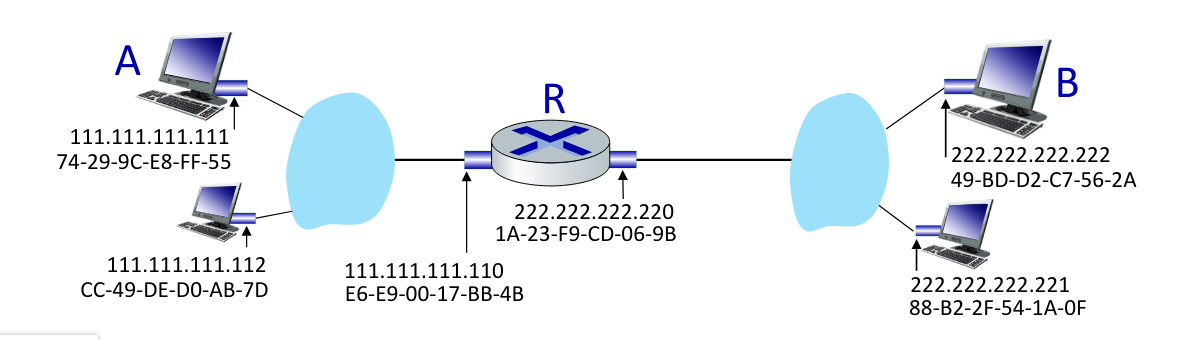
\includegraphics[width=\textwidth - 25pt]{images/MAC-Routing-Example.png}
        \item Every time a packet passes through a router, the source and destination MAC Addresses change.
    \end{itemize}

    \subsection*{Ethernet}
    \begin{itemize}
        \item \textbf{Ethernet} is the first \textbf{widely used Local Area Network (LAN) technology}.
        \item \textbf{Ethernet} is simple, cheap, and has a fast data transfer rate.
        \item Another bennified to \textbf{ethernet} is that \textbf{a single chip can support multiple transfer speeds}.
        \item Ways to implement ethernet connections:
        \begin{enumerate}
            \item \textbf{Bus} | A bus allows \textbf{several devices} to \textbf{communiate} with each other over a \textbf{single coaxial cable}. Such a implementation is susceptible to collision.
            \item \textbf{Switches} | A switch is a \textbf{physical device} that allows \textbf{several devices} to \textbf{connect to it over a physical link}. It then performs \textbf{switching}, which is essentially \textbf{forwarding frames} from one \textbf{node} to \textbf{another}. Such an implementation is not susceptible to collision.
        \end{enumerate}
        \item[] 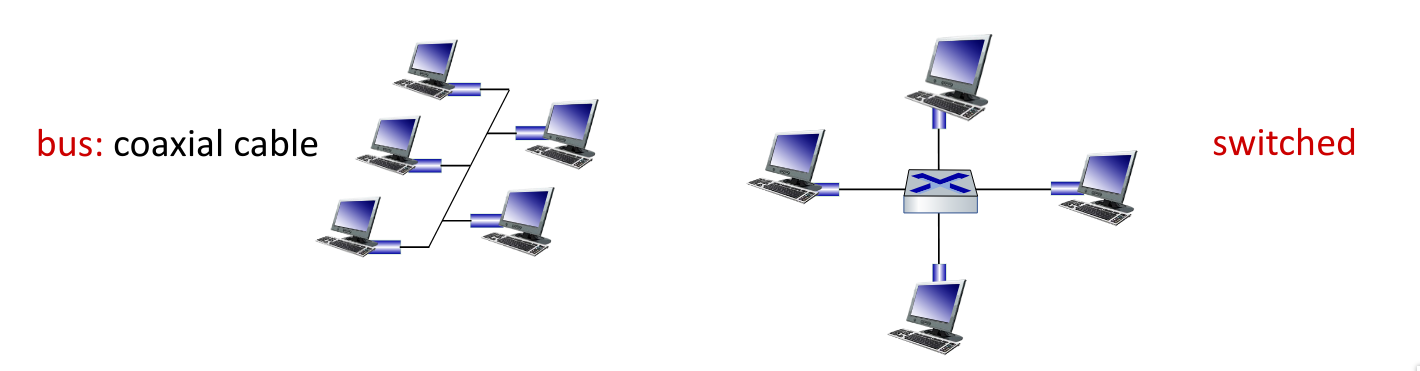
\includegraphics[width=\textwidth - 25pt]{images/Ethernet-Connections.png}
        \item \textbf{Using switches} is a modern way of \textbf{connecting devices on a LAN}.
        \item \textbf{Ethernet frames} consist of \textbf{six parts}:
        \begin{enumerate}
            \item \textbf{Preamble} | Preamble is used to synchronize sender and receiver clock rates. This consists of \textbf{7-bytes} of \textbf{10101010}, followed by one byte of \textbf{10101011}.
            \item \textbf{Destination Address} | The 6-byte destination MAC Address.
            \item \textbf{Source Address} | The 6-byte source MAC Address.
            \item \textbf{Type} | The type indicates the higher-level protocol (for example IP). This is also used to demultiplex at the receiver.
            \item \textbf{Payload} | The datagram.
            \item \textbf{CRC} | A cyclic redundancy check at the receiver. If an error is detected, the frame is dropped.
        \end{enumerate}
        \item \textbf{Ethernet proerties}:
        \begin{enumerate}
            \item \textbf{Connectionless} | No handshaking is performed between the sending and receiving NICs.
            \item \textbf{Unreliable} | The receiving NIC does not send ACKs or NAKs to the sending NIC. Dropped frames are only recovered if the inital sender uses a higher layer RDT (eg TCP).
            \item \textbf{MAC Protocol} | Ethernet's MAC protocol is the unslotted CSMA/CD with binary backoff.
        \end{enumerate}
        \item There are \textbf{many ethernet standards}, they all have the same \textbf{MAC protocol, and frame format}. However, they can \textbf{transmit data at different rates}.
    \end{itemize}

    \subsection*{Ethernet Switches}
    \begin{itemize}
        \item An \textbf{ethernet switch} is a \textbf{link-layer device} that takes an \textbf{active role}.
        \item \textbf{Ethernet switches} \textbf{store and forward ethernet frames}.
        \item \textbf{Ethernet switches} also examing the \textbf{MAC addresses} of \textbf{incoming frames}, and \textbf{selectively forward} the \textbf{frame} to \textbf{on or more outgoing links} via \textbf{CSMA/CD}.
        \item \textbf{Ethernet switches} are \textbf{transparent}; \textbf{nodes} are \textbf{unaware} of the \textbf{presence of switches}.
        \item \textbf{Ethernet switches} are \textbf{plug-and-play} and \textbf{self-learning}. They \textbf{do not} need to be \textbf{configured}.
        \item \textbf{Nodes} have a \textbf{direct, dedicated connection to switches}. This avoids collisions.
        \item \textbf{Ethernet switches} are \textbf{full duplex} with \textbf{buffering} used on the \textbf{incoming data} to \textbf{switches}.
        \item \textbf{Each ethernet switch} has a \textbf{switch table} that stores the \textbf{MAC address, interface number, and timestamp} or \textbf{each node} that is \textbf{connected to it}.
        \item As the \textbf{ethernet switch} is \textbf{self-learning} it can \textbf{learn} which \textbf{nodes} can be \textbf{reached}, and what \textbf{interfaces they can be reached through}. As it \textbf{learns this information}, it \textbf{stores it in the switch table}.
        \begin{itemize}
            \item There are two ways a switch can learn the MAC address of connected devices:
            \begin{enumerate}
                \item When a \textbf{frame} is sent to the \textbf{switch}, it contains a \textbf{source MAC address}, the switch "learns" that address, and adds it to the switch table.
                \item When a \textbf{frame} is sent to the \textbf{switch}, and has a \textbf{unmapped destination address}, it will \textbf{flood all interfaces} (except the sending interface), with the \textbf{frame} until one \textbf{responds}. Once a \textbf{node responds}, the \textbf{switch} will know that the \textbf{MAC address blongs to that node}.
            \end{enumerate}
        \end{itemize}
    \end{itemize}

    \subsection*{Switches vs Routers}
    \begin{itemize}
        \item \textbf{Routers} are \textbf{network-layer devices}.
        \item \textbf{Switches} are \textbf{link-layer devices}.
        \item \textbf{Routers} and \textbf{switches} both \textbf{store-and-forward} units of data.
    \end{itemize}

    \section*{\centering{Virtual Local Area Networks (VLANs)}}

    \subsection*{VLAN Motivation}
    \begin{itemize}
        \item If a \textbf{Local Area Network (LAN) scales} to a \textbf{very large size}, then all \textbf{layer-2 broadcast traffic} (ARP, DHCP, unknown MAC, etc) must cross the \textbf{entire LAN}.
        \item \textbf{Broadcast traffic} on a \textbf{large scale} can lead to \textbf{low efficiency} and \textbf{security / privacy issues}. 
        \item To overcome this issue, we can create \textbf{Virtual Local Area Networks (VLANs)}.
    \end{itemize}

    \subsection*{Port-Based VLANs}
    \begin{itemize}
        \item \textbf{Port-based Virtual Local Area Networks (VLANs)} can be configured so specific \textbf{port ranges} are part of specific \textbf{VLANs}. Effectively allowing a \textbf{single physical switch} to operate as \textbf{several virtual switches}.
        \item[] 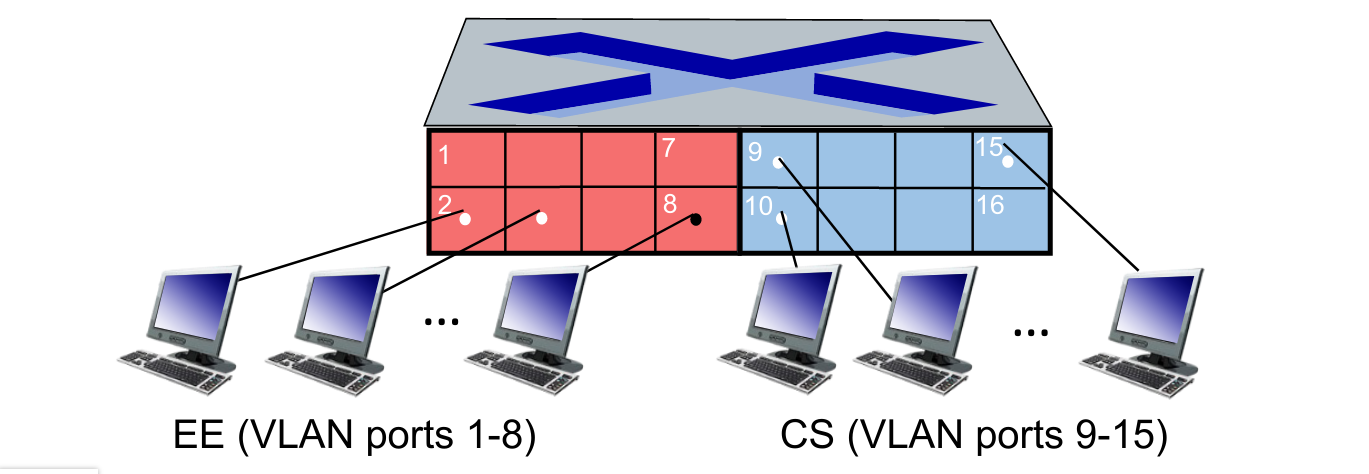
\includegraphics[width=\textwidth - 25pt]{images/VLAN.png}
        \item \textbf{Traffic isolation} refers to the \textbf{isolation of traffic within virtual networks}. The traffic within a virtual network cannot leave that network on layer 2.
        \item \textbf{Dynamic membership} refers to the \textbf{dynamic assigning of ports} among \textbf{VLANs}.
        \item \textbf{Forwarding between VLANs} can be done \textbf{via routing} through a \textbf{router}. In practice, vendors sell switches with build-in routers for this reason.
        \item \textbf{VLANs} that \textbf{span multiple switches} use \textbf{trunk ports} that \textbf{carry frames} between \textbf{VLANs} defined over \textbf{multiple physical switches}.
        \item[] 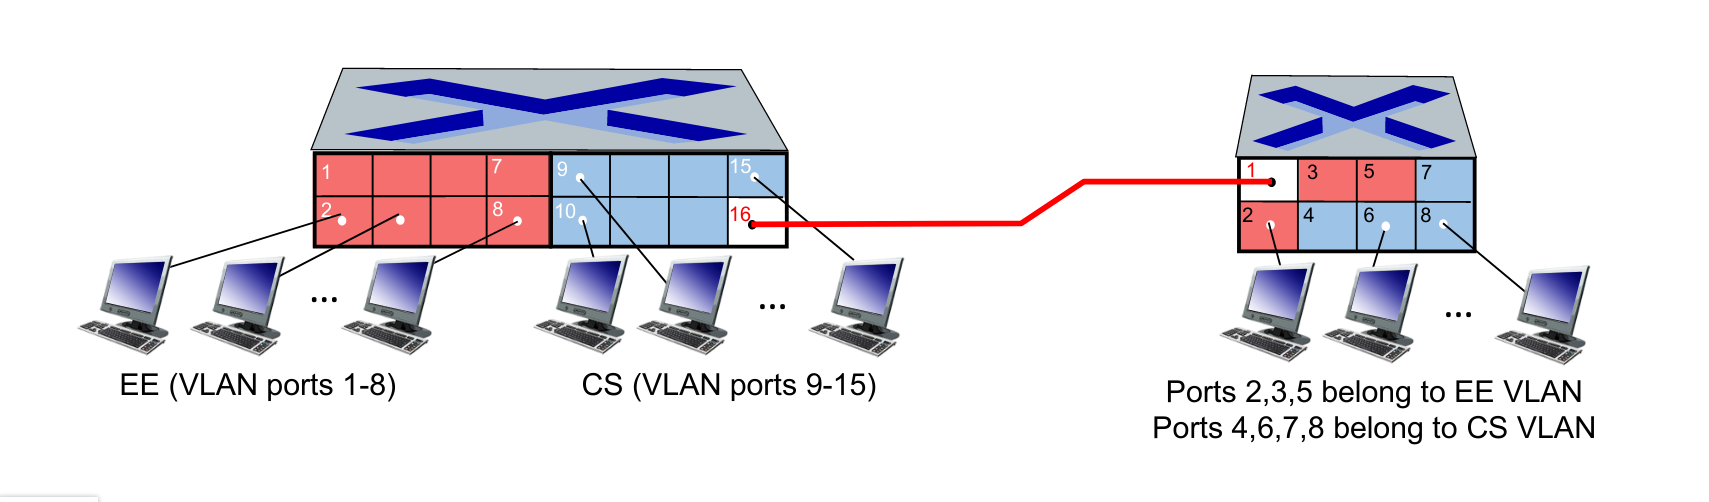
\includegraphics[width=\textwidth - 25pt]{images/Multi-VLANs.png} 
        \item A \textbf{problem} with \textbf{Port-Based VLANs} is that a \textbf{malicious actor} can \textbf{obtain access} to a \textbf{virtual network} simply by \textbf{connecting their device} to \textbf{one of the ports on the virtual network}.
        \begin{itemize}
            \item To get around this issue, \textbf{VLANs} can be defined by \textbf{device MAC addresses}. You simply \textbf{list all of the MAC addresses} that are a part of the \textbf{VLAN}.
        \end{itemize}
    \end{itemize}

\end{document}